\documentclass[11pt,a4paper]{article}
\usepackage[T1]{fontenc}
\usepackage{lmodern}
\usepackage[margin=22mm,headheight=15pt]{geometry}
\usepackage{graphicx}
\usepackage{booktabs,tabularx,array}
\usepackage{xcolor}
\usepackage{amsmath}
\usepackage{fancyhdr}
\usepackage{hyperref}
\usepackage{xurl}
\definecolor{navy}{HTML}{14243B}
\definecolor{blue}{HTML}{2A78D6}
\hypersetup{colorlinks=true,linkcolor=navy,urlcolor=blue,
  pdftitle={ExposureIQ: Content Exposure Intelligence},
  pdfauthor={Shubham Sharma and Ajay Singh},
  pdfsubject={CS404 Big Data Analytics: product pilot and historical research}}
\pagestyle{fancy}
\fancyhf{}
\fancyhead[L]{\small\textcolor{navy}{ExposureIQ}}
\fancyhead[R]{\small CS404 --- Big Data Analytics}
\fancyfoot[C]{\thepage}
\setlength{\parindent}{0pt}
\setlength{\parskip}{6pt}
\setlength{\emergencystretch}{2em}
\setcounter{tocdepth}{1}
\renewcommand{\arraystretch}{1.2}
\newcolumntype{Y}{>{\raggedright\arraybackslash}X}
\newcommand{\code}[1]{{\small\nolinkurl{#1}}}
\newcommand{\source}[1]{{\footnotesize\textit{Evidence:} \code{#1}\par}}
\newcommand{\chart}[2]{\begin{center}\includegraphics[width=\linewidth,height=0.36\textheight,keepaspectratio]{figures/#1}\par{\small #2}\end{center}}
\newcommand{\chapterpage}[1]{\clearpage\section{#1}}
\begin{document}
\begin{titlepage}
\color{navy}
{\large CS404 --- Big Data Analytics\par}
\vspace{25mm}
{\Huge\bfseries ExposureIQ\par}
\vspace{4mm}
{\LARGE Content Exposure Intelligence\par}
\vspace{10mm}
{\Large Distributed Analytics of Global Torrent Activity\par}
\vspace{4mm}
{\large A batch + streaming research platform and\\
an analyst-facing company pilot\par}
\vspace{18mm}
\begin{tabularx}{\linewidth}{@{}YY@{}}
\toprule
\textbf{Research foundation} & \textbf{Implemented product}\\
Public metadata, partitioned Parquet, Spark SQL and MLlib &
Catalogue approval, timestamped checks, investigations, alerts and reports\\
Historical collection: 10 October 2026 &
Localhost, single-process ExposureIQ pilot\\
\bottomrule
\end{tabularx}
\vfill
{\large\textbf{Team members}\par}
Shubham Sharma --- 2023BCS-062\\
Ajay Singh --- 2023BCS-004
\vspace{10mm}

October 2026\\
Aligned to the supplied \textit{Big Data Analytics} presentation
\vspace{8mm}

{\small Metadata only. Tracker observations are not unique people, verified
infringement, downloads or revenue loss. Historical findings are not live
product measurements.}
\end{titlepage}

\section*{Executive summary}
\addcontentsline{toc}{section}{Executive summary}
ExposureIQ turns a research pipeline over public torrent and entertainment
metadata into a local workspace for content-protection analysts. Film
distributors, streaming companies and game publishers can organise title
catalogues, review timestamped tracker observations, assign investigations
and export traceable records. The implemented product supports an analyst's
review process; it does not establish infringement or perform enforcement.

The research foundation, \textit{Distributed Analytics of Global Torrent
Activity}, combines batch preparation and a streaming speed layer. Apache
Spark cleans and joins RARBG, IMDb, TMDB, Steam and Wikipedia inputs into
Parquet. Public UDP tracker counters flow through Kafka and Spark Structured
Streaming to Parquet and PostgreSQL. Grafana supports the research dashboards;
FastAPI and SQLite support the ExposureIQ company workspace.

The archived research run contains 1,153,632,847 valid Wikipedia pageview rows,
2,843,691 RARBG catalogue records, 184,661,759 rows across four IMDb staging
tables, and 25,422,936 streamed observations. The latter were collected on
10 October 2026; the catalogue ends in May 2023. These time ranges must remain
visible when interpreting observations.

\begin{tabularx}{\linewidth}{@{}lY@{}}
\toprule
\textbf{Presentation query} & \textbf{Saved finding}\\
\midrule
Q1: Activity & Movie 1080p share rises from about 2\% to 62\% between 2008 and 2022.\\
Q2: Decay & Movie seeders follow a cross-sectional power-law association,
approximately $\mathrm{age}^{-0.73}$.\\
Q3: Release lag & Median first recorded cinema-to-listing lag is 9 days for
2020 and 2021 films in the selected sample.\\
Q4: Games & A logistic classifier of matched RARBG presence achieves test AUC 0.826.\\
Q5: Genres & Sci-Fi and Horror have positive listing-count residuals after
popularity/year adjustment.\\
Q6: Interest & Weekly Wikipedia views and seeders have movie Spearman correlation 0.472.\\
Bonus: Intraday & A fixed-panel study finds a game index range of about
11.4 points, with smaller movie/TV variation.\\
\bottomrule
\end{tabularx}

The company pilot adds explicit match approval, saved portfolio checks,
threshold rules, alerts, assigned cases, notes, exports and scheduled summary
snapshots. Company records are organisation-scoped; the research catalogue
and shared live collector are not private per-company streams.

All 26 entries in the archived validation file are labelled PASS. That is
not equivalent to every artefact being complete: the JSONL backup is 1,111
records short, a timestamp-boundary check has a recorded discrepancy, and
the original research Kafka topic was subsequently removed. This report
preserves those caveats.

\source{analysis/results/validation.csv; analysis/results/a1_* through a7_*}

\clearpage
\tableofcontents

\chapterpage{Problem, scope and product evolution}
\subsection{Research problem}
Torrent catalogues expose release metadata while public trackers report
swarm counters. Analysing these systematically requires reconciling
different identities, release dates, time ranges, formats and grains.
Individual listings are not the same as titles, and tracker counters from
overlapping swarms cannot be treated as independent audiences.

The project investigates how listing activity, release quality, release
timing, title age, game characteristics, genre and public interest relate
to the observed catalogue. Its scale includes over a billion pageview rows
and tens of millions of tracker events. Spark executes locally on the
project machine; this is distributed processing software in local mode,
not evidence of a deployed multi-node cluster.

\subsection{ExposureIQ's analyst-facing role}
The current product is \textbf{ExposureIQ: Content Exposure Intelligence}.
The academic subtitle remains useful because the presentation still
introduces the underlying research before describing the product.
ExposureIQ builds operational workflows around known titles and observations:
\begin{itemize}
\item Organise a company catalogue and explicitly approve proposed matches.
\item Request known-hash checks and inspect coverage, timestamp and failures.
\item Save portfolio observations and evaluate enabled threshold rules.
\item Assign investigations, record notes and export reviewable evidence.
\item Inspect a shared streaming pipeline and run bounded read-only queries.
\end{itemize}

The product does not continuously discover unknown new releases, verify
content ownership, submit takedowns, or measure legal damages. A successful
title match is a catalogue association, not an infringement determination.

\subsection{Compatibility, not a second brand}
User-facing names, report identity and exports use ExposureIQ. Existing
\code{CWATCH_*} settings, \code{/api/contentwatch} routes,
\code{X-CWatch-Request}, the \code{cwatch} PostgreSQL schema and the default
\code{cwatch.sqlite3} database remain compatibility identifiers.
Renaming those would require migrations for accounts, observations,
checkpoints and clients; a documentation refresh must not silently break
them.

The interface uses a dark, rounded visual theme with local assets. The
System Health page has been removed; minimal and administrator-only health
API endpoints remain. The public contact flow downloads an unsent enquiry
rather than claiming server-side delivery.

\source{portal/static/index.html; portal/static/contentwatch*.js; portal/server.py}

\chapterpage{Company workflows and evidence semantics}
\subsection{From import to investigation}
The demonstration sequence is \textbf{Import $\rightarrow$ Review
$\rightarrow$ Approve $\rightarrow$ Check $\rightarrow$ Investigate
$\rightarrow$ Report}. A company may also select individual titles directly
from the shared research catalogue.

CSV onboarding accepts unique \code{title,category} headers and an optional
\code{external_id}. The supported categories are movie, TV and game.
Imports are limited to 200 rows and 1 MB, and validation failure imports
nothing. Candidate matches remain pending until explicitly approved.
An imported name absent from the source catalogue does not become
monitorable merely because it was submitted.

Portfolio checks retain actual observation results. Ad-hoc search/check
operations are not automatically persisted as portfolio history. Users
must review timestamps, sampled hashes, responding trackers, missing
coverage and explicit failures. Counts use the maximum tracker-reported
seeders per record rather than a sum across overlapping trackers.

\begin{tabularx}{\linewidth}{@{}lY@{}}
\toprule
\textbf{Record} & \textbf{Meaning and limitation}\\
\midrule
Catalogue entry & Company title and approval decision; not a tracker measurement.\\
Saved check & Timestamped known-hash observations and coverage; not complete discovery.\\
Rule / alert & Enabled threshold applied to a qualifying fresh check; not legal risk scoring.\\
Investigation & Assigned human review with state and notes; not automated enforcement.\\
Export & A traceable snapshot of records; generation time is not observation time.\\
\bottomrule
\end{tabularx}

\subsection{Access, alerts and reporting}
Administrators manage company access and operate the shared live collector.
Analysts manage workflows and may run permitted live queries. Viewers and
read-only API keys may inspect/export authorised records but cannot mutate
company workflows. Private records are scoped to the current organisation.

An enabled title-specific rule should exist before a demonstration check.
Unavailable or stale checks do not trigger rules, and an unresolved alert
for the same rule/title suppresses duplicates. Optional email/webhook
delivery has recorded states and errors; configured delivery is not proof
that a notification arrived.

Reports include actual saved company summaries, catalogue CSV, observation
CSV, complete check JSON and print-to-PDF workflows. Scheduled daily/weekly
UTC summaries persist once per current period while the portal runs; they
do not backfill missed periods. Signing out preserves records and does not
stop the collector. Personal watchlists remain browser-local.

\source{portal/accounts.py; portal/company.py; docs/EXPOSUREIQ_PILOT.md}

\chapterpage{Architecture and separation of concerns}
\begin{center}
\fbox{\begin{minipage}{0.92\linewidth}
\textbf{Batch:} public source dumps / APIs\\
$\downarrow$ acquisition and validation\\
Raw files $\rightarrow$ Spark cleaning $\rightarrow$ staging Parquet\\
$\downarrow$ identity joins and research aggregates\\
Curated Parquet $\rightarrow$ Spark SQL / MLlib $\rightarrow$ saved results\\[5pt]
\textbf{Speed:} public UDP tracker counts\\
$\downarrow$ metadata scraper\\
Kafka $\rightarrow$ Spark Structured Streaming\\
$\downarrow$ separate lake and serving queries\\
Parquet event history + PostgreSQL snapshots / aggregates / batch ledger\\[5pt]
\textbf{Serving:} Grafana research dashboards + FastAPI ExposureIQ API\\
$\downarrow$ company authentication and workflow operations\\
SQLite company state + browser workspace / exports
\end{minipage}}
\end{center}

The batch layer provides historical context and title associations.
The speed layer retains newly observed counters. PostgreSQL serves bounded
queries over snapshots and aggregates, while Parquet retains larger event
history. SQLite stores private operational records rather than duplicating
the entire research lake.

Three collection contexts are distinct: the historical research run,
the ExposureIQ product stream and the resettable classroom demo.
The product uses topic \code{tracker.scrapes.cwatch}, schema
\code{cwatch} and dedicated Parquet/checkpoint paths. Its starter creates
three Kafka partitions. The presentation's six-partition configuration
describes the research topic, not a universal product configuration.

Kafka, PostgreSQL, Grafana and optional scraper services are configured
through Docker Compose. Spark runs on local cores. The original research
environment was a 12-core machine with approximately 15 GB RAM; the report
does not claim cluster benchmarks or horizontal scalability measurements.

The product's \textbf{Query} editor executes PostgreSQL over
\code{live_latest}, \code{live_minutes} and \code{live_batches}.
Research examples in \code{demo.sql} use Spark SQL. These engines, views
and result grains must not be conflated.

\source{infra/docker-compose.yml; streaming/swarm_stream.py; portal/live.py}

\chapterpage{Data sources, time coverage and identities}
\begin{tabularx}{\linewidth}{@{}Yrl@{}}
\toprule
\textbf{Source / prepared surface} & \textbf{Saved rows} & \textbf{Coverage}\\
\midrule
Wikipedia valid hourly pageviews & 1,153,632,847 & 1--7 Sep 2026\\
IMDb: four staging tables & 184,661,759 & Research snapshot\\
RARBG catalogue & 2,843,691 & 2007--May 2023\\
Steam games after deduplication & 125,854 & Oct 2026 snapshot\\
TMDB title records & 13,462 & Selected titles\\
TMDB release-date records & 212,933 & Selected titles\\
Historical stream observations & 25,422,936 & 10 Oct 2026\\
Full-catalogue tracker scan & 1,385,068 & 10 Oct 2026\\
\bottomrule
\end{tabularx}

Counts describe distinct surfaces and are not additive estimates of unique
people or titles. IMDb's total refers to basics, alternative titles,
principals and episodes. The roughly 1.38-billion-row research description
is a scale summary, not a deduplicated entity count.

The presentation contains an approximate 1.5-billion pageview statement;
its source list and archived validation support
\textbf{1,153,632,847 valid pageview rows}. This report uses the latter
rather than propagating inconsistent rounding.

\subsection{Identity resolution}
A torrent's \code{infohash} identifies one release. IMDb IDs join film/TV
metadata to release dates; Steam app IDs identify games. Multiple release
hashes can map to one title. Wikipedia entities are matched by page title
and confidence, using English desktop/mobile views for the interest study.
The product's \code{title_key} identifies a title, not a torrent.

Game name normalisation associates about 79\% of relevant game torrents
with Steam entries. The presentation reports 34 correct matches in a
35-item manual check; this is a small spot check, not a population-wide
accuracy guarantee. Unmatched games affect model outcome labels.

\subsection{Dates are part of the evidence}
The RARBG catalogue stops in May 2023. Tracker measurements were collected
in October 2026, while the Wikipedia week is in September 2026. A chart
combining these sources is not a contemporaneous user-behaviour panel.
On-demand product checks carry their own actual timestamps.

\source{analysis/results/validation.csv; dataset/README.md; docs/schema.md}

\chapterpage{Preparation, streaming and reproducibility}
\subsection{Batch preparation}
Raw inputs are retained separately from cleaned staging and joined curated
tables. Spark writes compressed, partitioned Parquet for the research lake.
Release-name parsing extracts title, year, season/episode, resolution,
codec and source. The presentation records \code{guessit} parsing through
\code{mapInPandas} on 12 workers, taking about 60 minutes for the RARBG
catalogue; this is an archived run observation, not a current benchmark.

Cleaning includes infohash deduplication, normalisation of catalogue
categories, tolerant casting, malformed-line handling and explicit Steam
CSV schema repair. The Steam header has 39 names for 40 values because
Discount and DLC count were merged. Wikipedia loses 93,017 malformed lines
out of 1,153,725,864 raw lines (about 0.0081\%); these are excluded, not
silently treated as valid pageviews.

Exact IMDb identifiers support film/TV joins; normalised names support
Steam associations. Broadcast joins reduce large pageview scans against
small title lookup tables. The presentation reports about one minute for
its selected Wikipedia title join; it does not establish end-to-end
pipeline latency.

\subsection{Stream processing and replay}
Scrapers request public tracker counters using BEP 15 UDP scrape messages.
They do not request peer lists. Kafka JSON includes hash, tracker, seeders,
leechers, completed count and observation timestamp. Spark parses events
and excludes rows lacking a usable hash or timestamp.

One query appends Parquet; another applies serving micro-batches.
The serving transaction inserts a query/batch ledger record and updates
minute summaries and latest observations together. A replayed ledger key
is skipped, avoiding duplicate serving application for that batch.
Latest observations are keyed by infohash/tracker and updated using
timestamp order.

The two sinks have separate progress/checkpoint state. Transactional
serving replay protection is not a blanket claim of atomicity across
Kafka, Parquet, PostgreSQL and JSONL. Kafka retention, checkpoint loss,
input drops and forced shutdown still need operational handling.

\subsection{A lightweight report rebuild}
The replacement charts read tracked result CSVs and reuse the repository's
plot style. Rebuilding this PDF does not rerun Spark, acquire datasets,
contact trackers, change results or read company records. It therefore
reproduces the presentation of saved evidence, not the original experiment.
Full research validation requires the prepared lake and appropriate services.

\source{etl/; ingest/; streaming/swarm_stream.py; analysis/render_saved.py}

\chapterpage{Q1: Activity and release quality (A1)}
\textbf{Question.} How have upload volume and release quality changed by
category? The study groups catalogue records by upload year, then derives
movie resolution and codec shares from parsed release names.

\chart{a1_uploads_by_year.png}{Upload counts describe listings, not unique titles or downloads.}

\begin{center}
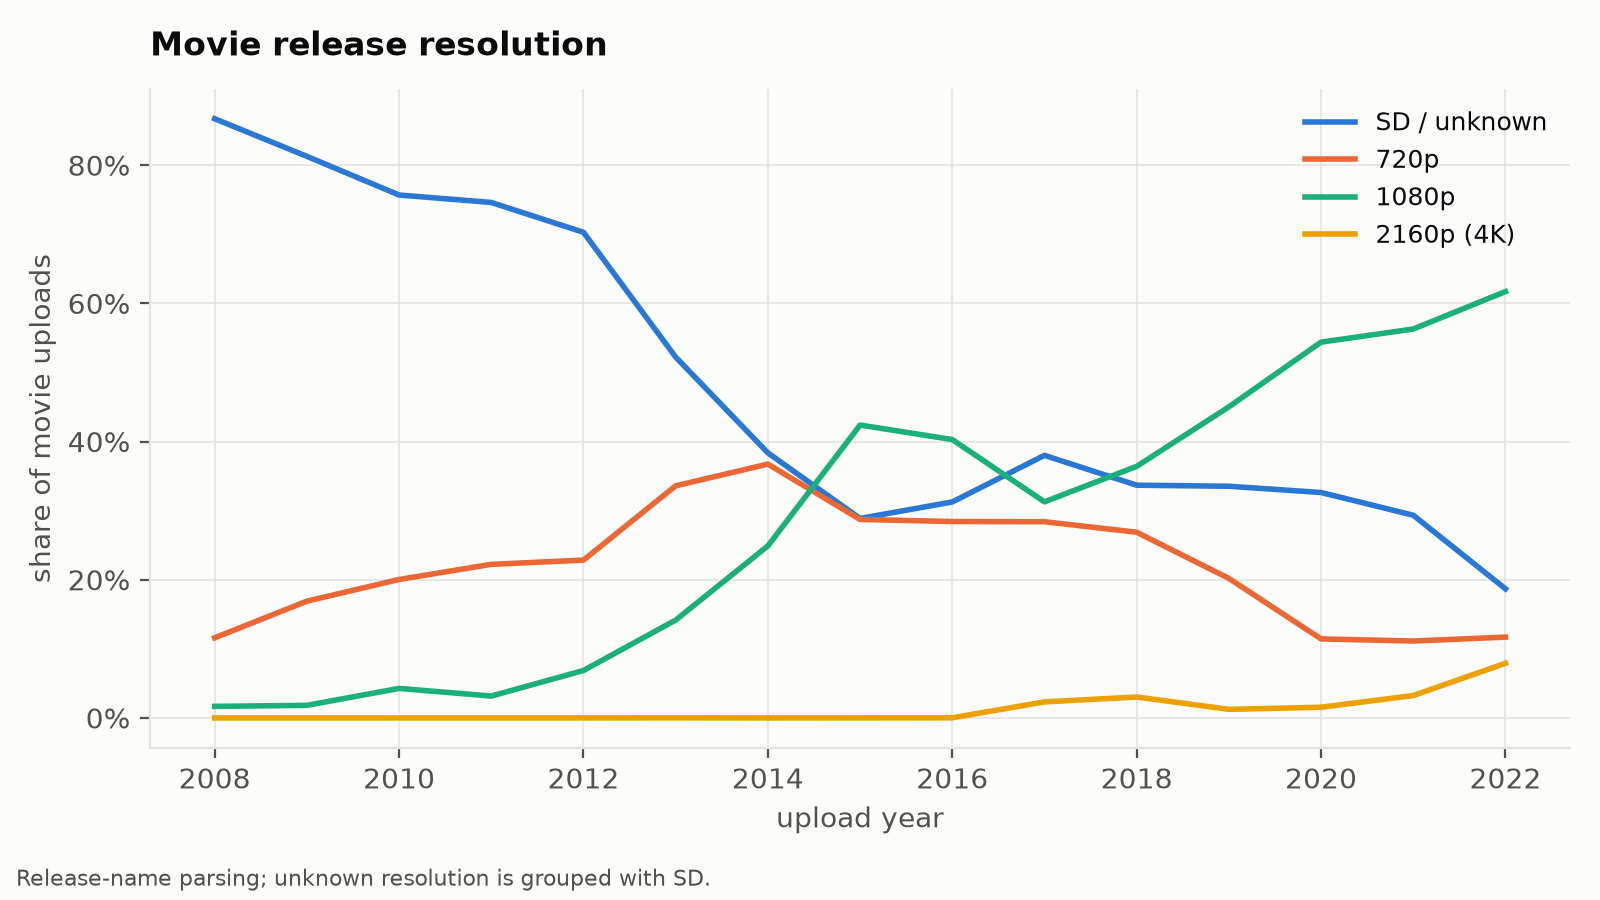
\includegraphics[width=0.49\linewidth]{figures/a1_movie_resolution.png}
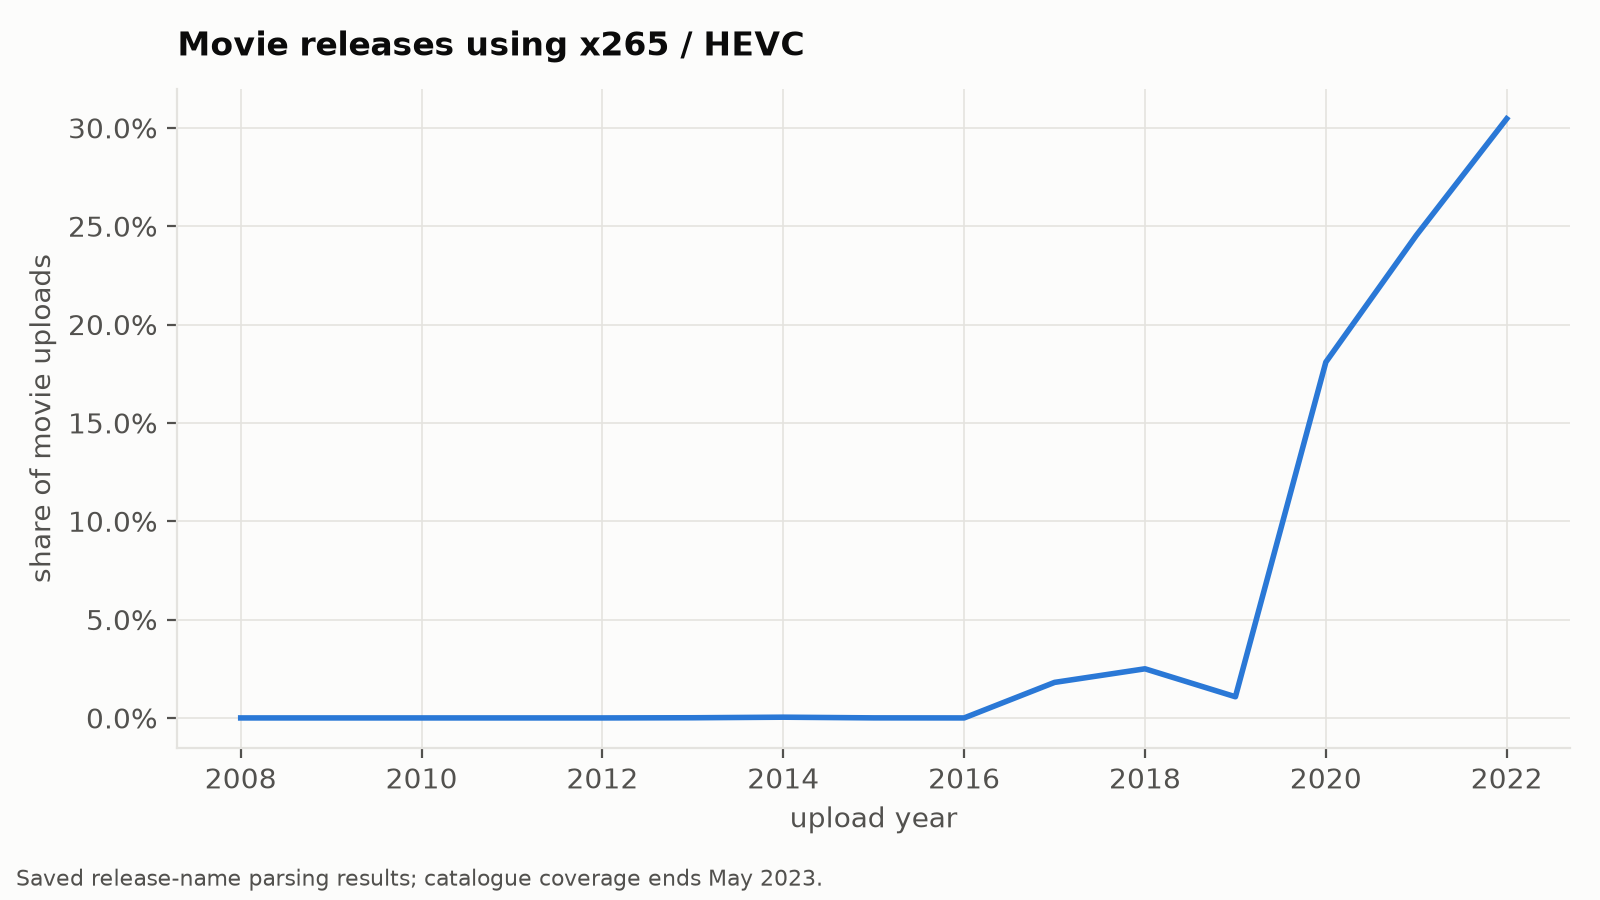
\includegraphics[width=0.49\linewidth]{figures/a1_movie_x265.png}
\end{center}

TV uploads rise from 1,068 in 2010 to roughly 80,000--100,000 per year over
2018--2022. Movie 1080p share increases from about 2\% in 2008 to 62\% in 2022;
x265/HEVC share increases from about 1\% in 2019 to 30\% in 2022.
Different formats and repacks can represent the same underlying title.

\textbf{Analyst use.} These trends provide historical context for release
formats and catalogue composition. They do not establish which formats a
current rights holder should prioritise without current, licensed evidence.

\textbf{Limits.} RARBG is one catalogue; removed releases and site-specific
listing practices affect counts. 2023 ends in May and must not be compared
as a full year. Parsed labels can be missing or ambiguous.

\source{analysis/results/a1_uploads_by_category_year.csv}
\source{analysis/results/a1_movie_resolution_share.csv; a1_movie_x265_share.csv}

\chapterpage{Q2: Popularity decay and persistence (A3)}
\textbf{Question.} How does observed swarm size vary with title age?
The research aggregates seeders across versions per title, then fits
Poisson generalised linear models for exponential and power-law forms.
The selected fit population uses title release years 2012--2023.

\[
\log E[S \mid a] = \beta_0+\beta_1 a
\quad\hbox{or}\quad
\log E[S \mid a] = \beta_0+\beta_1\log a .
\]

\chart{a3_decay.png}{Cross-sectional scan: title release cohorts are not longitudinal trajectories.}

\begin{tabularx}{\linewidth}{@{}lrY@{}}
\toprule
\textbf{Category} & \textbf{Titles} & \textbf{Best saved fit by AIC}\\
\midrule
Movie & 34,632 & Power law: coefficient $-0.733$; AIC 401,682.94\\
TV & 10,301 & Power law: coefficient $+1.647$; no negative decay association\\
Game & 10,871 & Exponential: coefficient $+0.157$; positive age association\\
\bottomrule
\end{tabularx}

For films, the exponential alternative has AIC 402,250.00, about 567 points
higher. The preferred association is approximately
$S\propto a^{-0.73}$. The positive TV/game fits must not be described as
negative decay; continuing series and persistent older games may contribute.

\textbf{Analyst use and limits.} The result motivates attention to long-lived
known titles. It does not predict an individual title's future trajectory.
Survivorship, missing old listings, title matching and version splitting
remain. The presentation's 9.0\% alive-torrent figure describes the archived
full-scan cross-section, not a current product success rate.

\source{analysis/results/a3_title_decay_fits.csv; a3_title_decay_by_release_year.csv}

\chapterpage{Q3: Release-to-listing lag (A2)}
\textbf{Question.} How soon after cinema and legal home release do films
appear in the recorded catalogue? The first surviving RARBG listing per
film is compared with TMDB release dates. The selected movie window is
2018 through 31 March 2023; older release cohorts are too incomplete to
support the same interpretation.

\chart{a2_leak_vs_home_ecdf.png}{Zero marks legal home release; a negative lag is an earlier recorded listing.}

\begin{tabularx}{\linewidth}{@{}lrrY@{}}
\toprule
\textbf{Year} & \textbf{Films} & \textbf{Median days} & \textbf{Interpretation}\\
\midrule
2018 & 429 & 76 & Cinema to first surviving listing\\
2019 & 411 & 75 & Cinema to first surviving listing\\
2020 & 322 & 9 & Shorter observed lag\\
2021 & 367 & 9 & Shorter observed lag\\
2022 & 363 & 18 & Selected catalogue sample\\
2023 & 61 & 19 & Partial release-year coverage\\
\bottomrule
\end{tabularx}

The presentation reports 66--70\% of the 2020--2023 cohort listed by the
day after legal home release, and a one-day median from TV series premiere
to the first recorded series torrent. ``Home'' means the earliest qualifying
digital or physical date, not necessarily a single worldwide launch date.

\textbf{Analyst use.} Release windows can guide when analysts review known
titles. They are not a guarantee of automated early discovery.

\textbf{Limits.} First surviving catalogue listing is not independently
verified first online availability. Country-specific windows, replacements,
missing listings and incomplete matching can change lags. The historical
pattern is not evidence that every present-day release leaks within one day.

\source{analysis/results/a2_movie_first_upload.csv; a2_movie_leak_by_year.csv; a2_tv_first_upload.csv}

\chapterpage{Q4: Game characteristics and catalogue presence (A5)}
\textbf{Question.} How do price, popularity and game type relate to the
presence of a matched RARBG listing? The population is Steam games released
2018--2022 with at least 100 reviews. The study label ``pirated'' means
at least one matched RARBG game torrent; it does not verify every underlying
file or legal status.

\chart{a5_pirated_by_band.png}{Descriptive proportions by price and review-count band; these are not causal price effects.}

The logistic model uses standardised features, an 80/20 split with seed 42,
and regularisation. Test AUC is \textbf{0.8263}, rounded to 0.83 in the
presentation. Odds ratios are per one standard deviation of each feature,
not a per-dollar effect.

\begin{tabularx}{\linewidth}{@{}Yr@{}}
\toprule
\textbf{Feature} & \textbf{Approximate odds ratio / SD}\\
\midrule
Popularity (log reviews) & 1.84\\
Single-player & 1.79\\
Price (log transformed) & 1.55\\
Massively multiplayer & 0.77\\
Casual & 0.71\\
Free-to-play & 0.54\\
Early Access & 0.51\\
\bottomrule
\end{tabularx}

Free-to-play titles have about 5.4\% matched presence; \$5--40 bands have
roughly 52--54\%. The above-\$40 band is 37.5\% but contains only
\textbf{32 games}, so the apparent decline deserves caution.

\textbf{Analyst use and limits.} These associations support contextual
prioritisation, not individual guilt or causal pricing recommendations.
Unmatched torrents create incomplete outcome labels. The split evaluates
held-out catalogue labels, not unseen future markets or production alerts.

\source{analysis/results/a5_logit_pirated.csv; a5_pirated_by_band.csv; analysis/a5_games.py}

\chapterpage{Q5: Genre associations beyond popularity (A6)}
\textbf{Question.} Which film genres have more recorded versions than their
popularity and release year would predict? The study fits an OLS model of
log listing counts and summarises residuals by genre:
\[
\log(1+\text{torrents}) \sim \log(\text{IMDb votes})
  + \text{release-year indicators}.
\]
The displayed effect is $\exp(\text{mean residual})-1$.

\chart{a6_genre_excess_piracy.png}{Residual-based associations; genres overlap and are not randomised treatments.}

The saved result gives approximately \textbf{Sci-Fi +59\%},
\textbf{Horror +56\%}, \textbf{Romance $-18$\%} and
\textbf{Comedy $-12$\%}. The model's saved $R^2$ is 0.1933:
most variation remains unexplained. A residual effect is not the fraction
of a genre's audience engaged in infringement.

\textbf{Analyst use.} Genre can provide background context for a catalogue
review queue when combined with actual company titles, current observations
and human judgement. ExposureIQ does not turn these research coefficients
into an automatically validated legal risk score.

\textbf{Limits.} IMDb votes are a popularity proxy and may correlate with
unmeasured factors. Genre memberships overlap, catalogue selection is
incomplete and residual summaries do not establish causality.
Multiple versions and release practices can affect the count outcome.

\source{analysis/results/a6_genre_excess_piracy.csv; a6_model.csv; analysis/a6_genres.py}

\chapterpage{Q6: Public interest and observed seeders (A4)}
\textbf{Question.} Does Wikipedia interest track the observed torrent
activity of matched titles? The study compares weekly English Wikipedia
views with seeders using Spearman rank correlation.

\chart{a4_wiki_vs_seeders.png}{Rebuilt correlation summary from the saved results, not a new scatter-plot experiment.}

\begin{tabularx}{\linewidth}{@{}lrrY@{}}
\toprule
\textbf{Category} & \textbf{Matched titles} & \textbf{Spearman $\rho$} & \textbf{Reading}\\
\midrule
Movie & 41,901 & 0.4718 & Moderate positive rank association\\
TV & 8,422 & 0.4056 & Moderate positive rank association\\
Game & 3,273 & 0.2394 & Weaker positive rank association\\
\bottomrule
\end{tabularx}

The three samples sum to 53,596 titles. Correlation is far from one, so
public interest is only a partial proxy for observed swarm activity.
It is not a conversion rate from pageviews to downloads.

\textbf{Analyst use.} Interest metadata can contextualise why a title may
attract attention, but fresh timestamped checks are needed to describe
current tracker responses. The product should not label a title as
currently exposed solely because it is popular.

\textbf{Limits.} Wikipedia matching can be ambiguous, and English
desktop/mobile views are not global demand. The interest week and the
tracker collection are not simultaneous. Both signals may reflect other
causes, including marketing or legal release timing.

\source{analysis/results/a4_spearman.csv; analysis/a4_wiki_interest.py}

\chapterpage{Bonus: Swarms during one day (A7)}
\textbf{Question.} How does observed swarm size vary within the research
collection day? The design uses opentrackr only, a fixed panel and
20-minute windows to reduce tracker-outage and changing-sample artefacts.
Each torrent is indexed relative to its own daily mean before averaging.

\chart{a7_swarm_day.png}{The chart retains stored IST window labels; a window start may precede the observation cutoff.}

\begin{tabularx}{\linewidth}{@{}lrrr@{}}
\toprule
\textbf{Category} & \textbf{Min index} & \textbf{Max index} & \textbf{Mean leechers/seeder}\\
\midrule
Movie & 99.11 & 100.65 & 0.354\\
TV & 99.59 & 100.55 & 0.416\\
Game & 95.04 & 106.43 & 0.236\\
\bottomrule
\end{tabularx}

The index range is 1.54 points for movies, 0.96 for TV and 11.40 for games.
The game's range is not automatically an 11.4\% increase from its first
observation. The presentation's ``+11\%'' is a rounded description of this
intraday pattern, not a demonstrated repeatable daily cycle.

The observation cutoff is 12:40--20:50 IST on 10 October 2026.
Spark window alignment can produce an earlier displayed slot label; labels
must not be mistaken for observations outside the filter. Panel eligibility
requires observations in at least 90\% of slots and positive median seeders;
slots need at least 80\% panel coverage.

\textbf{Analyst use and limits.} The result illustrates why sampling design
matters for dashboards. A one-day, selected alive-torrent panel cannot
establish global time-zone behaviour or a general daily seasonality model.
Tracker counters remain partial observations, not unique users.

\source{analysis/results/a7_panel_by_slot.csv; a7_summary.csv; analysis/a7_swarm_day.py}

\chapterpage{Validation, performance and evidence quality}
\subsection{What the archived checks establish}
The saved file has 26 PASS-labelled entries, including source/staging
reconciliation, hash uniqueness, 168 Wikipedia hourly files, count sanity,
cross-tracker agreement and selected parsing/release-date spot checks.
They are recorded results from the original experiment, not freshly
executed checks during this report rebuild.

\begin{tabularx}{\linewidth}{@{}YY@{}}
\toprule
\textbf{Archived measurement} & \textbf{Result and scope}\\
\midrule
Kafka / serving ledger / Parquet & Each records 25,422,936 observations for the historical run.\\
Duplicate serving application & Zero recorded duplicate micro-batches; 603 committed batches.\\
Tracker agreement & Spearman 0.736 on selected cross-tracker pairs.\\
Full scan versus near-time live scrape & Spearman 0.977 on selected same-tracker pairs.\\
Presentation peak throughput & Approximately 3.56 million rows/hour; not an end-to-end latency SLA.\\
Total research collection & About 10.4 hours; 25.4 million observations.\\
\bottomrule
\end{tabularx}

\subsection{Caveats that PASS labels do not erase}
\textbf{JSONL backup shortfall.} The backup has 25,421,825 lines, which is
1,111 fewer than Kafka/Parquet. Its note attributes the difference to an
unflushed write buffer when scraper containers were force-stopped.
Thus ``zero lost'' in the presentation applies to the reconciled primary
pipeline, not every secondary backup.

\textbf{Timestamp envelope.} The archived boundary check lists an expected
05:06--15:31 UTC envelope and an observed 05:05--15:30 UTC range, yet is
marked PASS. This report records the discrepancy rather than claiming an
exactly satisfied boundary test.

\textbf{Removed source topic.} Kafka totals reference an offset snapshot
recorded on 10 October 2026; the original topic was later removed.
The tracked snapshot supports historical provenance but cannot substitute
for querying a still-existing original topic.

\textbf{Product versus research testing.} Unit tests cover company and
portal behaviour separately. Saved research validation is not a substitute
for verifying current authentication, isolation, live startup, failure
handling and exports. A report build is not a production certification.

\source{analysis/results/validation.csv; kafka_offsets_snapshot.json; portal/test_*.py}

\chapterpage{Operating, demonstrating and preserving the project}
\subsection{Start the existing pilot}
With prepared dependencies and research data, run from the repository root:
\begin{verbatim}
uv run python -m portal.server
# http://localhost:8800
\end{verbatim}
Create a company or sign in. Do not reacquire datasets, rerun ETL or reset a
classroom stream just to open the website. The administrator can start
known-hash monitoring with 100, 500 or 2,000 targets. Docker, Java and
populated historical PostgreSQL serving data are required for shared streaming.

The product's query connection is a dedicated non-superuser read-only
PostgreSQL login with a five-second statement timeout, one-second lock
timeout and 200-row cap. Include observation-time filters when asking about
fresh records. Retained snapshots remain queryable after collection stops.

\subsection{Rebuild the report and run checks}
\begin{verbatim}
uv run python -m analysis.render_saved
latexmk -pdf -interaction=nonstopmode -halt-on-error \
  -cd report/ExposureIQ_Report.tex
uv run python -m unittest discover -s portal -p 'test_*.py'
\end{verbatim}
The supplied presentation is preserved separately under \code{showcase/}.
The report's editable LaTeX, rendered PDF, charts and saved research CSVs
are suitable tracked artefacts. Company records are not.

\subsection{Backup before reclaiming disk space}
A Git push preserves tracked repository content only. It does not preserve
the ignored data lake, the company database, credentials, the local ZIP,
browser watchlists or Docker-backed Kafka/PostgreSQL/Grafana state.
Checkpoints preserve processing progress, not the full observation history.

Use the provided SQLite backup API rather than copying only an active
database main file:
\begin{verbatim}
uv run python -m portal.manage backup \
  --file /safe/private/location/exposureiq.sqlite3
\end{verbatim}
Stop the portal before restore. The restore tool invalidates sessions,
revokes API keys and marks invitations used. Keep private backups outside
the public checkout. Neither chart generation nor PDF compilation needs
dataset deletion or cache cleanup.

\source{portal/manage.py; docs/EXPOSUREIQ_PILOT.md; report/README.md}

\chapterpage{Limitations, ethics and conclusion}
\subsection{Measurement limits}
RARBG represents one catalogue ending in May 2023, not the whole torrent
ecosystem. Public trackers observe only part of each swarm. Counts can
overlap across trackers and releases and do not identify people.
Unknown hashes are outside the current product's monitoring scope.
Matching errors, incomplete release dates and removed old listings affect
all downstream conclusions.

The decay study is cross-sectional, not a repeated observation of every
title over its lifespan. The intraday study covers one selected panel on
one day. Game labels depend on incomplete name matching. Wikipedia interest
is language- and period-specific. Regression and correlation findings
describe associations, not causal effects.

\subsection{Privacy and responsible use}
The implementation analyses metadata and tracker counters, not copyrighted
media content. Scrapers do not request peer lists or store peer IP
addresses. Company records and credentials remain private and excluded
from source control. Analysts must retain timestamps, coverage and
limitations when sharing observations; an alert is a review prompt,
not a finding against an individual.

Public accessibility does not remove source licence obligations. In
particular, IMDb inputs are non-commercial. Any commercial deployment
requires review and replacement/licensing of unsuitable sources.
Source terms and lawful use must be evaluated before expanding collection.

\subsection{Pilot boundaries and future work}
ExposureIQ currently runs as a single-process localhost pilot. Shared
stream ownership and reader credentials are managed in process memory.
There is no billing, MFA, account recovery or email verification service.
Internet deployment requires HTTPS, stronger operational safeguards,
recovery procedures and validation under the intended tenant/deployment
model. No production-readiness or enforcement claim is made.

Potential future work includes licensed contemporary catalogue sources,
evaluated discovery mechanisms, longer longitudinal studies, robust
deployment/recovery and better matching evaluation. These are future
requirements, not implemented product features.

\subsection{Conclusion}
The project connects large-scale historical research with a concrete
analyst workflow. ExposureIQ makes title decisions, observations and human
review more traceable while preserving the original six research questions
and intraday streaming study. Its credibility depends on separating
historical findings from fresh checks, public metadata from private company
state, and measured associations from legal or causal conclusions.

\chapterpage{Evidence map and references}
\subsection{Presentation order and implementation}
\begin{tabularx}{\linewidth}{@{}llY@{}}
\toprule
\textbf{Deck} & \textbf{Module} & \textbf{Tracked result evidence}\\
\midrule
Q1 Activity & A1 & Upload counts, resolution shares, codec shares\\
Q2 Decay & A3 & Release-cohort aggregates, model coefficients and AIC\\
Q3 Release lag & A2 & First listings, yearly summaries, TV lag\\
Q4 Games & A5 & Standardised odds ratios, AUC, price/review bands\\
Q5 Genres & A6 & OLS coefficients and genre residual summaries\\
Q6 Interest & A4 & Category sample sizes and Spearman correlations\\
Bonus Intraday & A7 & Fixed-panel slot observations and category summaries\\
\bottomrule
\end{tabularx}

Research source and CSVs are under \code{analysis/} and
\code{analysis/results/}. The product implementation is under \code{portal/};
stream processing is under \code{streaming/}. The data/identity reference
and operator guide are under \code{docs/}. The report's build instructions
are \code{report/README.md}.

\subsection{Supplied presentation}
\textit{Big Data Analytics}, Shubham Sharma and Ajay Singh, CS404.
User-supplied October 2026 PDF, preserved as
\texttt{showcase/Big\ Data\ Analytics.pdf}. The presentation retains the academic
project title and introduces ExposureIQ as the intended analyst workspace.
Its research charts and rounded claims are interpreted alongside saved
result tables, not as evidence of new measurements.

\subsection{Prior work cited in the presentation}
\begin{enumerate}
\item Pouwelse et al. (2005), BitTorrent measurement, availability and
flash crowds, IPTPS. Presentation reference:
\url{https://pdos.csail.mit.edu/archive/6.824-2007/papers/pouwelse-btmeasure.pdf}.
\item Guo et al. (2005), torrent popularity and peer-to-peer measurement,
IMC. Presentation reference:
\url{https://static.usenix.org/event/imc05/tech/full_papers/guo/guo.pdf}.
\item Meulpolder et al. (2010), \textit{Public and Private BitTorrent
Communities: A Measurement Study}, IPTPS.
\url{https://www.usenix.org/conference/iptps-10/public-and-private-bittorrent-communities-measurement-study}.
\item Zhang et al. (2011), public BitTorrent ecosystem measurement,
IEEE TPDS. Presentation reference:
\url{https://cse.engineering.nyu.edu/~ross/papers/PublicEcosystem.pdf}.
\end{enumerate}

\subsection{Source and protocol references}
IMDb non-commercial datasets: \url{https://datasets.imdbws.com/}.\\
Wikimedia hourly pageviews: \url{https://dumps.wikimedia.org/other/pageviews/}.\\
TMDB developer API: \url{https://developer.themoviedb.org/}.\\
Steam dataset (fronkongames):
\url{https://www.kaggle.com/datasets/fronkongames/steam-games-dataset}.\\
BEP 15 UDP tracker protocol:
\url{https://www.bittorrent.org/beps/bep_0015.html}.

\end{document}
